%introduction used to set the whole 

\documentclass{article}
\title{hw4}
\author{Wenhua Bao 2512664\\Xinrui Chen 2503398}
\usepackage{graphicx}
\usepackage{pdfpages}
\usepackage{amsmath}
\usepackage{amssymb}

%TEXT
\begin{document}
\maketitle
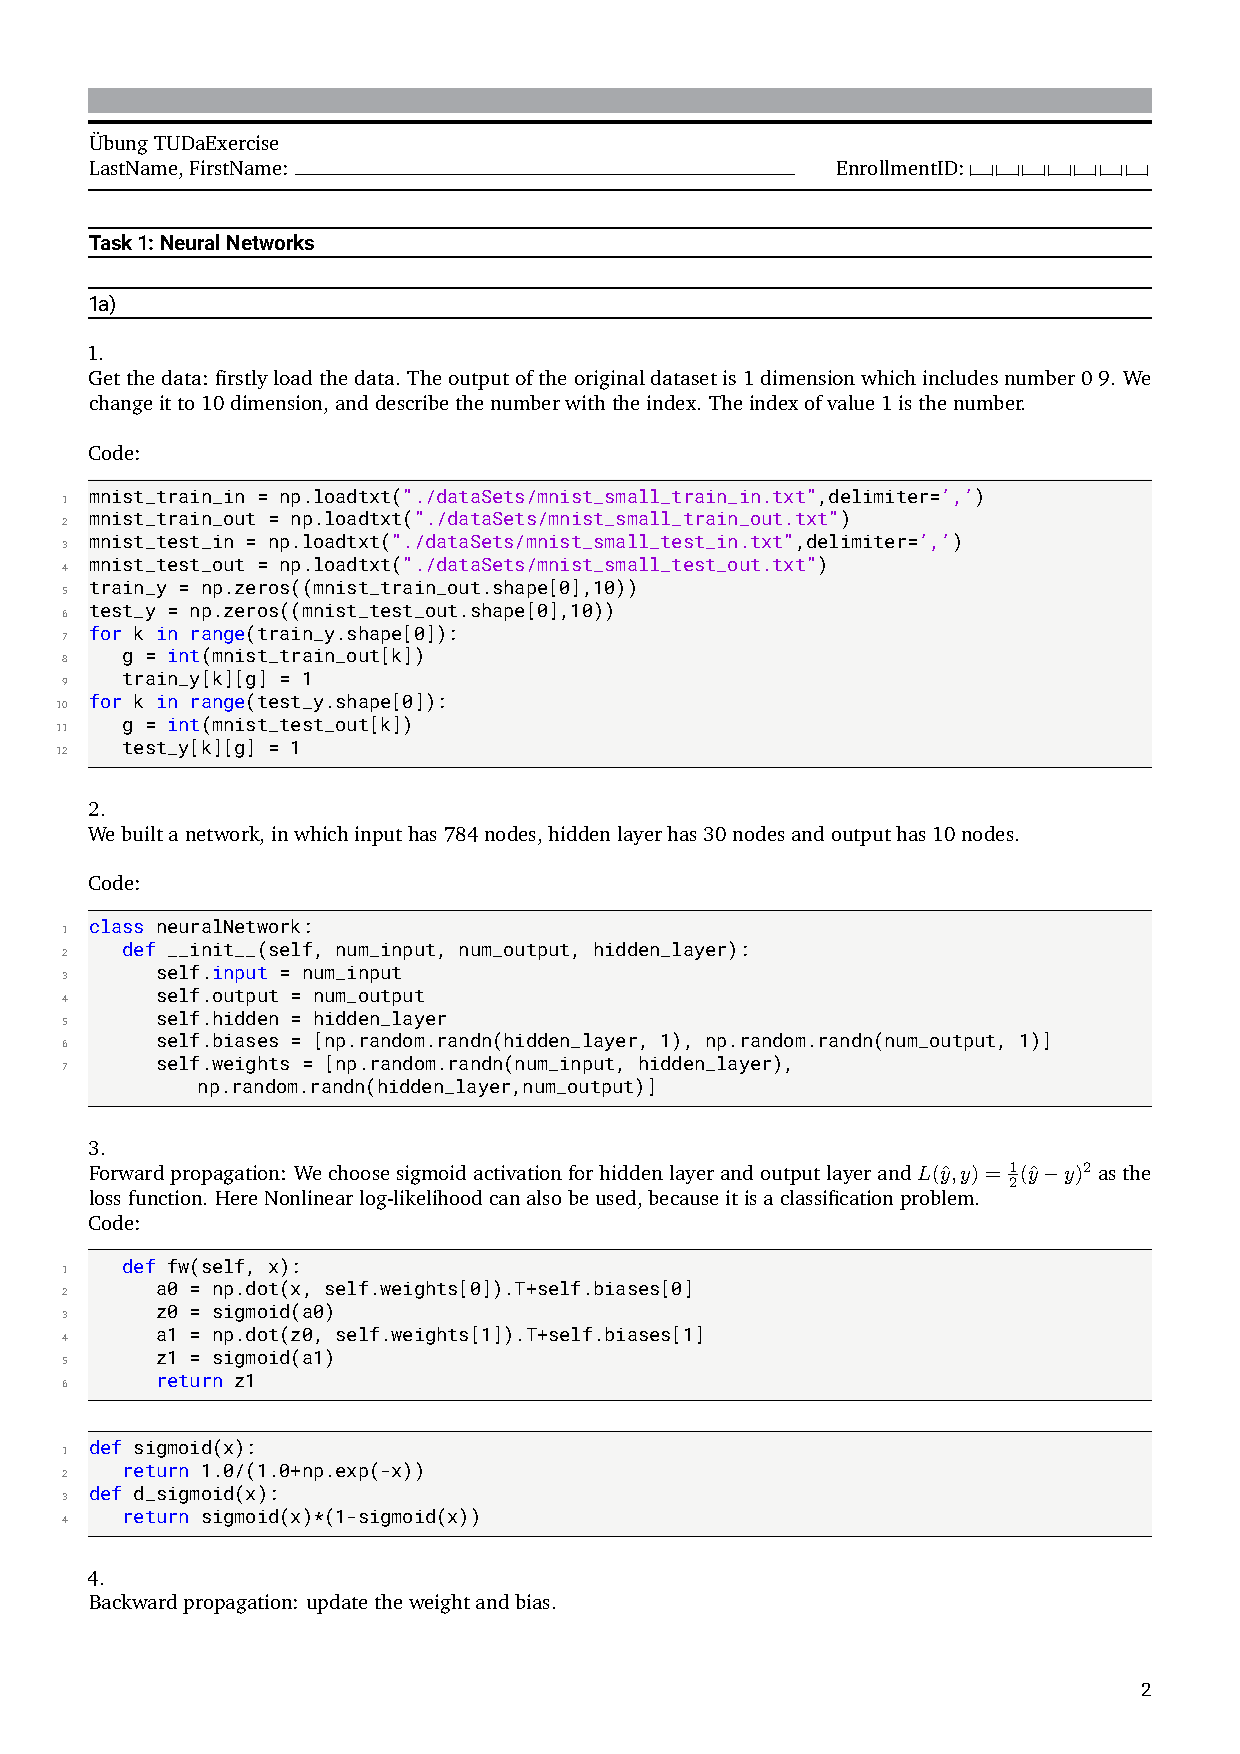
\includepdf[pages={-}]{hw4cc.pdf}
\section{Task2}
\subsubsection{a}
1. SVM is the linear classifier with the largest spacing defined on the feature space .
2.Advantages: The classifier only depends on a few data points.
              Both the original SVM formulation (primal) as well as the
              derived dual formulation are quadratic programming problems
              (quadratic cost, linear constraints), which have unique solutions
              that can be computed efficiently
\subsubsection{b}
$$\begin{aligned}
\arg \min _{w, b} & \frac{1}{2}\|w\|^{2} \\
\text { s.t. } & y_{i}\left(w^{\top} x_{i}+b\right)-1 \geqslant 0 \quad \forall i
\end{aligned}$$
\subsubsection{c}
In reality the modes have noise to make models not linear separable, slack variables make the model can tolerant noise and become linear separable.
$$\begin{array}{l}
\arg min \frac{1}{2}\|w\|^{2}+C \sum_{i=1}^{N} \zeta_{i} \\
\text { sit. } y_{i}\left(w^{\top} x_{i}+b\right) \geqslant 1-s_{i} \quad(i=1,2, \ldots N) \\
\zeta_{i} \geqslant 0
\end{array}$$
\subsubsection{d}
$$\begin{array}{c}
\left.L(\omega, b, \alpha)=\frac{1}{2}\|w\|^{2}-\alpha_{i} \sum_{i=1}^{N} ( y_{i}\left(w^{\top} x_{i}+b\right)-1\right) \\
=\frac{1}{2}\|w\|^{2}-\sum_{i=1}^{N} \alpha_{i} y_{i} w^{\top} x_{i}-\sum_{i=1}^{N} \alpha_{i} y_i b+\sum_{i=1}^{N} \alpha_{i} \\
\frac{\partial L}{\partial w}=w-\sum \alpha_{i} y_{i} x_{i}=0 \\
w=\sum \alpha_{i} y_{i} x_{i} \\
\frac{\partial L}{\partial b}=-\sum \alpha_{i} y_{i}=0 \\
\sum \alpha_{i} y_{i}=0
\end{array}$$
$$\begin{aligned}
L(w, b, \alpha) &=\frac{1}{2} \sum_{i=1}^{N} \sum_{j=1}^{N} \alpha_{i} \alpha_{j} y_{i} y_{j}\left(x_{j}^{\top} x_{i}\right)-\sum_{i=1}^{N} \sum_{j=1}^{N} \alpha_{i} a_{j} y_{i} y_{j}\left(x_{j}^{\top} x_{i}\right)+\sum_{i=1}^{N} a_{i} \\
&=\sum_{i=1}^{N} a_{i}-\frac{1}{2} \sum_{i=1}^{N} \sum_{j=1}^{N} \alpha_{i} \alpha_{j} y_{i} y_{j}\left(x_{j}^{\top} x_{i}\right)
\end{aligned}$$
result
$$\begin{aligned}
\min \sum_{i=1}^{N} \alpha_{i}-\frac{1}{2} \sum_{i=1}^{N} \sum_{j=1}^{N} \alpha_{i} \alpha_{j} y_{i} y_{j}\left(x_{i}^{\top} x_{j}\right) \\
\text { s.t. } \alpha_{i} \geqslant 0 \\
\sum_{i=1}^{N} \alpha_{i} y_{i}=0
\end{aligned}$$
\subsubsection{e}
we can skip the derivation
\subsubsection{f}
1.Replace every occurrence of a scalar product between features with a kernel function
$$K\left(\mathbf{x}_{i}, \mathbf{x}_{j}\right)=\phi\left(\mathbf{x}_{i}\right)^{\top} \phi\left(\mathbf{x}_{j}\right)$$
2.A kernel $K\left(\mathbf{x}_{i}, \mathbf{x}_{j}\right)$that allows us to compute the
scalar product without making the mapping explicit
\subsubsection{g}

\section{Task3}
\subsection{a}
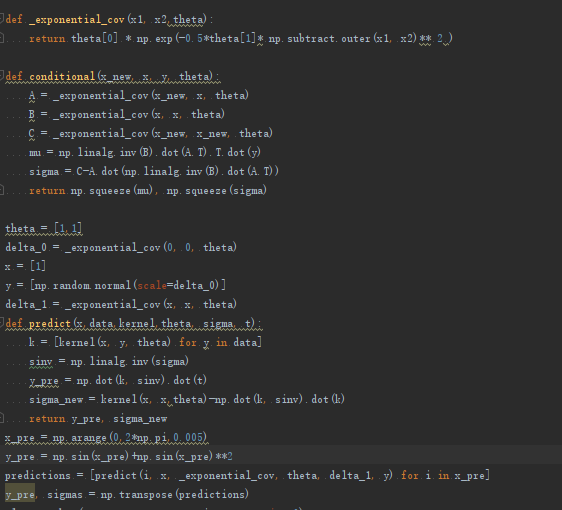
\includegraphics[width=0.45\textwidth]{1596403073(1).png}
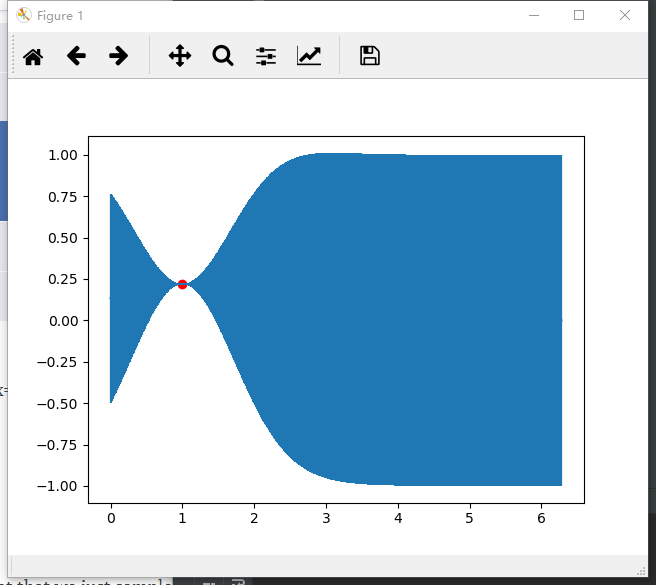
\includegraphics[width=0.45\textwidth]{1596402750(1).png}
\end{document}